% Options for packages loaded elsewhere
\PassOptionsToPackage{unicode}{hyperref}
\PassOptionsToPackage{hyphens}{url}
\documentclass[
  11pt,
]{article}
\usepackage{xcolor}
\usepackage[margin=1in]{geometry}
\usepackage{amsmath,amssymb}
\setcounter{secnumdepth}{5}
\usepackage{iftex}
\ifPDFTeX
  \usepackage[T1]{fontenc}
  \usepackage[utf8]{inputenc}
  \usepackage{textcomp} % provide euro and other symbols
\else % if luatex or xetex
  \usepackage{unicode-math} % this also loads fontspec
  \defaultfontfeatures{Scale=MatchLowercase}
  \defaultfontfeatures[\rmfamily]{Ligatures=TeX,Scale=1}
\fi
\usepackage{lmodern}
\ifPDFTeX\else
  % xetex/luatex font selection
\fi
% Use upquote if available, for straight quotes in verbatim environments
\IfFileExists{upquote.sty}{\usepackage{upquote}}{}
\IfFileExists{microtype.sty}{% use microtype if available
  \usepackage[]{microtype}
  \UseMicrotypeSet[protrusion]{basicmath} % disable protrusion for tt fonts
}{}
\makeatletter
\@ifundefined{KOMAClassName}{% if non-KOMA class
  \IfFileExists{parskip.sty}{%
    \usepackage{parskip}
  }{% else
    \setlength{\parindent}{0pt}
    \setlength{\parskip}{6pt plus 2pt minus 1pt}}
}{% if KOMA class
  \KOMAoptions{parskip=half}}
\makeatother
\usepackage{longtable,booktabs,array}
\newcounter{none} % for unnumbered tables
\usepackage{calc} % for calculating minipage widths
% Correct order of tables after \paragraph or \subparagraph
\usepackage{etoolbox}
\makeatletter
\patchcmd\longtable{\par}{\if@noskipsec\mbox{}\fi\par}{}{}
\makeatother
% Allow footnotes in longtable head/foot
\IfFileExists{footnotehyper.sty}{\usepackage{footnotehyper}}{\usepackage{footnote}}
\makesavenoteenv{longtable}
\usepackage{graphicx}
\makeatletter
\newsavebox\pandoc@box
\newcommand*\pandocbounded[1]{% scales image to fit in text height/width
  \sbox\pandoc@box{#1}%
  \Gscale@div\@tempa{\textheight}{\dimexpr\ht\pandoc@box+\dp\pandoc@box\relax}%
  \Gscale@div\@tempb{\linewidth}{\wd\pandoc@box}%
  \ifdim\@tempb\p@<\@tempa\p@\let\@tempa\@tempb\fi% select the smaller of both
  \ifdim\@tempa\p@<\p@\scalebox{\@tempa}{\usebox\pandoc@box}%
  \else\usebox{\pandoc@box}%
  \fi%
}
% Set default figure placement to htbp
\def\fps@figure{htbp}
\makeatother
\setlength{\emergencystretch}{3em} % prevent overfull lines
\providecommand{\tightlist}{%
  \setlength{\itemsep}{0pt}\setlength{\parskip}{0pt}}
\usepackage{float}
\usepackage{bookmark}
\IfFileExists{xurl.sty}{\usepackage{xurl}}{} % add URL line breaks if available
\urlstyle{same}
\hypersetup{
  pdftitle={Evaluation Statistics},
  hidelinks,
  pdfcreator={LaTeX via pandoc}}

\title{Evaluation Statistics}
\author{}
\date{\vspace{-2.5em}}

\begin{document}
\maketitle

{
\setcounter{tocdepth}{2}
\tableofcontents
}
\section{Setup}\label{setup}

\subsection{Import and Filter Data}\label{import-and-filter-data}

\begin{longtable}[]{@{}
  >{\raggedright\arraybackslash}p{(\linewidth - 4\tabcolsep) * \real{0.0899}}
  >{\raggedright\arraybackslash}p{(\linewidth - 4\tabcolsep) * \real{0.7303}}
  >{\raggedleft\arraybackslash}p{(\linewidth - 4\tabcolsep) * \real{0.1798}}@{}}
\caption{Entries excluded by timeout, minimum-duration, and dependency
filtering.}\tabularnewline
\toprule\noalign{}
\begin{minipage}[b]{\linewidth}\raggedright
phase
\end{minipage} & \begin{minipage}[b]{\linewidth}\raggedright
removal\_reason
\end{minipage} & \begin{minipage}[b]{\linewidth}\raggedleft
removed\_entries
\end{minipage} \\
\midrule\noalign{}
\endfirsthead
\toprule\noalign{}
\begin{minipage}[b]{\linewidth}\raggedright
phase
\end{minipage} & \begin{minipage}[b]{\linewidth}\raggedright
removal\_reason
\end{minipage} & \begin{minipage}[b]{\linewidth}\raggedleft
removed\_entries
\end{minipage} \\
\midrule\noalign{}
\endhead
\bottomrule\noalign{}
\endlastfoot
Phase 5 & Elapsed time exceeded configured timeout plus grace period &
5 \\
R3 & Recovery execution below 10 seconds; treated as not run & 2 \\
R4 & Elapsed time exceeded configured timeout plus grace period & 1 \\
R5 & Dependent recovery or stability entry removed with primary phase &
3 \\
R5 & Recovery execution below 10 seconds; treated as not run & 89 \\
SR & Dependent recovery or stability entry removed with primary phase &
3 \\
\end{longtable}

\subsection{Theme Settings}\label{theme-settings}

\section{Success Rates}\label{success-rates}

\begin{longtable}[]{@{}lr@{}}
\caption{Number of Valid Runs Recorded for Each Evaluation
Phase}\tabularnewline
\toprule\noalign{}
Phase & Number of runs \\
\midrule\noalign{}
\endfirsthead
\toprule\noalign{}
Phase & Number of runs \\
\midrule\noalign{}
\endhead
\bottomrule\noalign{}
\endlastfoot
Phase 1 & 236 \\
S1 & 106 \\
R1 & 130 \\
Phase 2.1 & 235 \\
Phase 2.2 & 234 \\
Phase 3 & 233 \\
S3 & 222 \\
R3 & 9 \\
Phase 4 & 228 \\
S4 & 133 \\
R4 & 94 \\
Phase 5 & 221 \\
S5 & 107 \\
R5 & 27 \\
SR & 238 \\
\end{longtable}

\subsection{Final Outcome by Main
Phase}\label{final-outcome-by-main-phase}

\begin{center}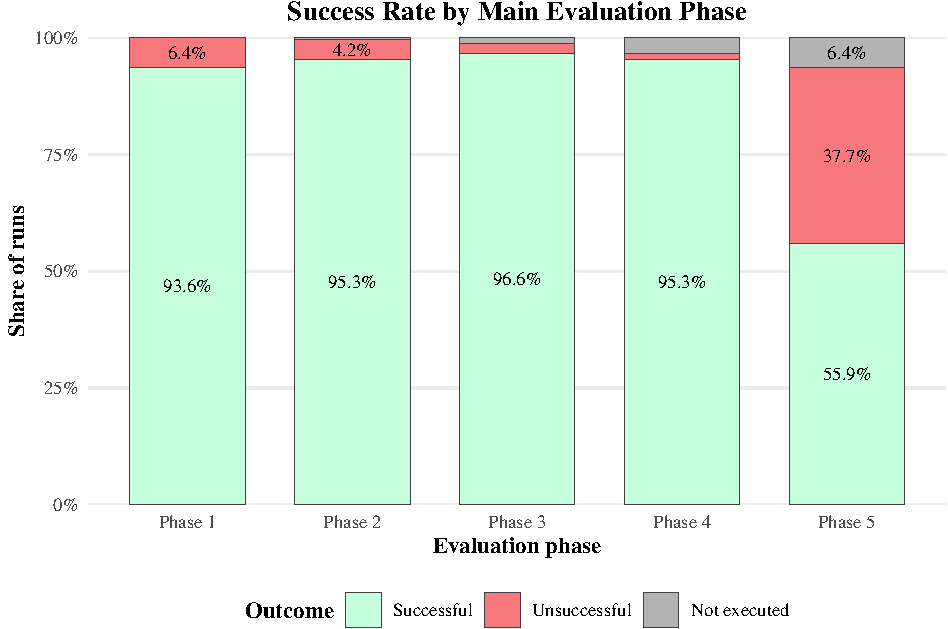
\includegraphics{figures/final-success-rate-chart-1} \end{center}

\subsection{Direct, Recovered, Failed, and Not-Run
Outcomes}\label{direct-recovered-failed-and-not-run-outcomes}

\begin{center}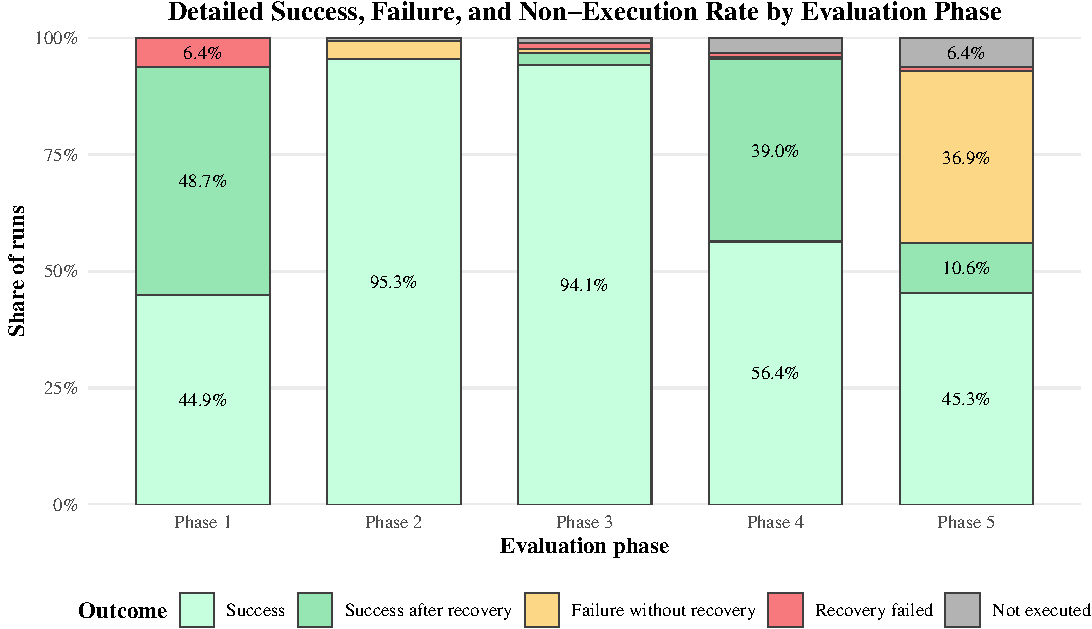
\includegraphics{figures/detailed-outcome-chart-1} \end{center}

\begin{longtable}[]{@{}
  >{\raggedright\arraybackslash}p{(\linewidth - 10\tabcolsep) * \real{0.1071}}
  >{\raggedleft\arraybackslash}p{(\linewidth - 10\tabcolsep) * \real{0.1964}}
  >{\raggedleft\arraybackslash}p{(\linewidth - 10\tabcolsep) * \real{0.2143}}
  >{\raggedleft\arraybackslash}p{(\linewidth - 10\tabcolsep) * \real{0.0714}}
  >{\raggedleft\arraybackslash}p{(\linewidth - 10\tabcolsep) * \real{0.1964}}
  >{\raggedleft\arraybackslash}p{(\linewidth - 10\tabcolsep) * \real{0.2143}}@{}}
\caption{Run counts by phase outcome, including phases that were not
executed.}\tabularnewline
\toprule\noalign{}
\begin{minipage}[b]{\linewidth}\raggedright
phase\_group
\end{minipage} & \begin{minipage}[b]{\linewidth}\raggedleft
Failure (no recovery)
\end{minipage} & \begin{minipage}[b]{\linewidth}\raggedleft
Failure (with recovery)
\end{minipage} & \begin{minipage}[b]{\linewidth}\raggedleft
Not run
\end{minipage} & \begin{minipage}[b]{\linewidth}\raggedleft
Success (no recovery)
\end{minipage} & \begin{minipage}[b]{\linewidth}\raggedleft
Success (with recovery)
\end{minipage} \\
\midrule\noalign{}
\endfirsthead
\toprule\noalign{}
\begin{minipage}[b]{\linewidth}\raggedright
phase\_group
\end{minipage} & \begin{minipage}[b]{\linewidth}\raggedleft
Failure (no recovery)
\end{minipage} & \begin{minipage}[b]{\linewidth}\raggedleft
Failure (with recovery)
\end{minipage} & \begin{minipage}[b]{\linewidth}\raggedleft
Not run
\end{minipage} & \begin{minipage}[b]{\linewidth}\raggedleft
Success (no recovery)
\end{minipage} & \begin{minipage}[b]{\linewidth}\raggedleft
Success (with recovery)
\end{minipage} \\
\midrule\noalign{}
\endhead
\bottomrule\noalign{}
\endlastfoot
Phase 1 & 0 & 15 & 0 & 106 & 115 \\
Phase 2 & 9 & 0 & 2 & 225 & 0 \\
Phase 3 & 2 & 3 & 3 & 222 & 6 \\
Phase 4 & 1 & 2 & 8 & 133 & 92 \\
Phase 5 & 87 & 2 & 15 & 107 & 25 \\
\end{longtable}

\section{Final Success Rate by Input
Variables}\label{final-success-rate-by-input-variables}

\subsection{Phase 1: Initial Network
Formation}\label{phase-1-initial-network-formation}

\begin{center}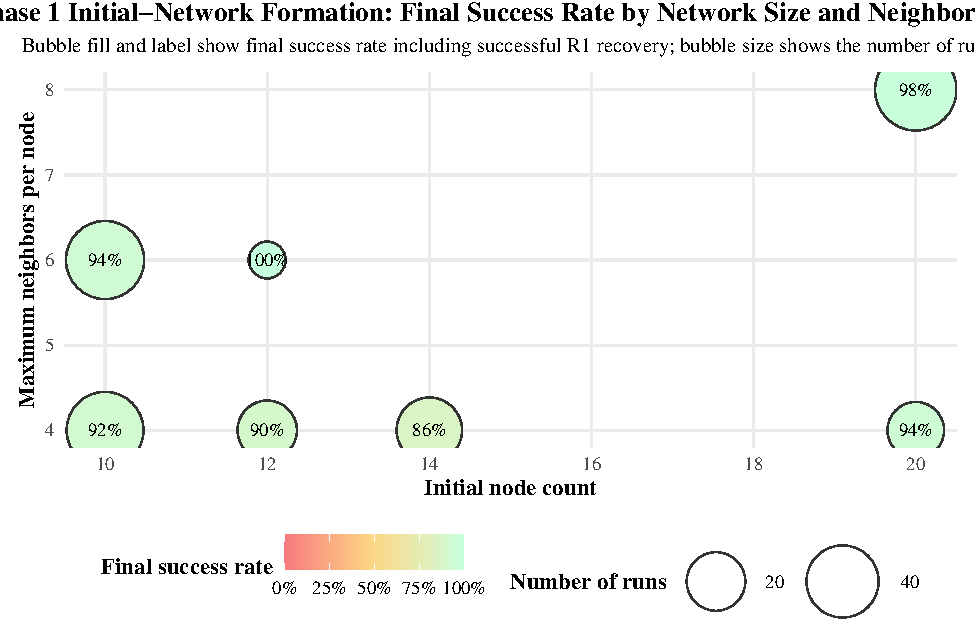
\includegraphics{figures/phase1-input-chart-1} \end{center}

\subsection{Phase 3: Single-Node Failure
Repair}\label{phase-3-single-node-failure-repair}

\begin{center}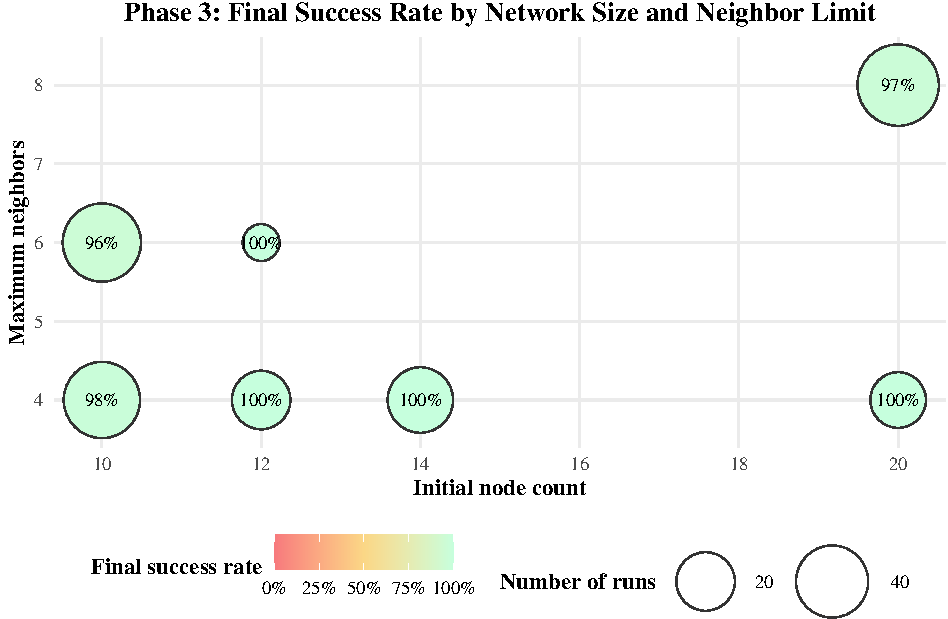
\includegraphics{figures/phase3-input-chart-1} \end{center}

\subsection{Phase 4: Adding Nodes}\label{phase-4-adding-nodes}

\begin{center}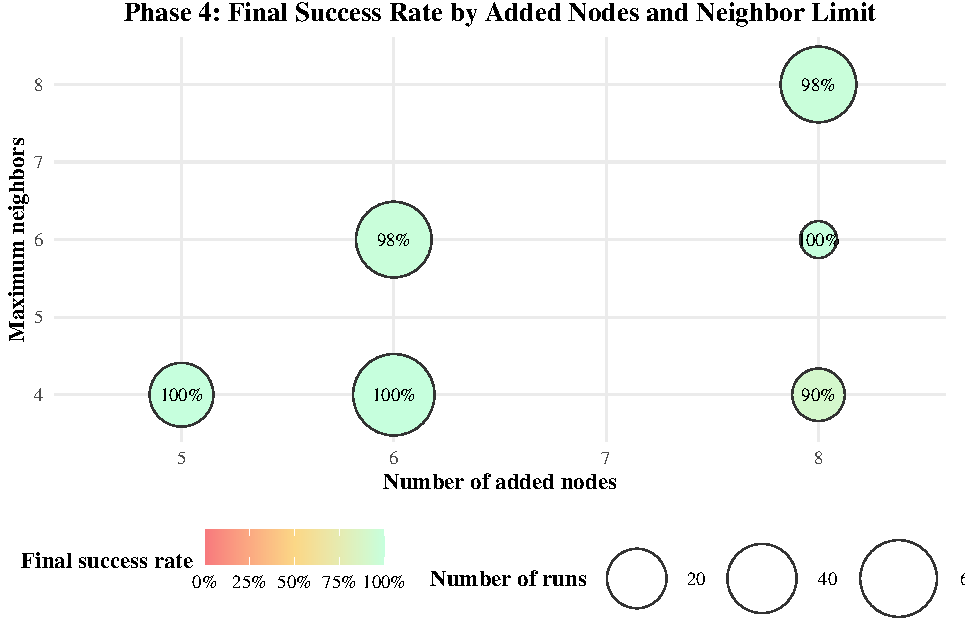
\includegraphics{figures/phase4-input-chart-1} \end{center}

\subsection{Phase 5: Removing Multiple
Nodes}\label{phase-5-removing-multiple-nodes}

\begin{center}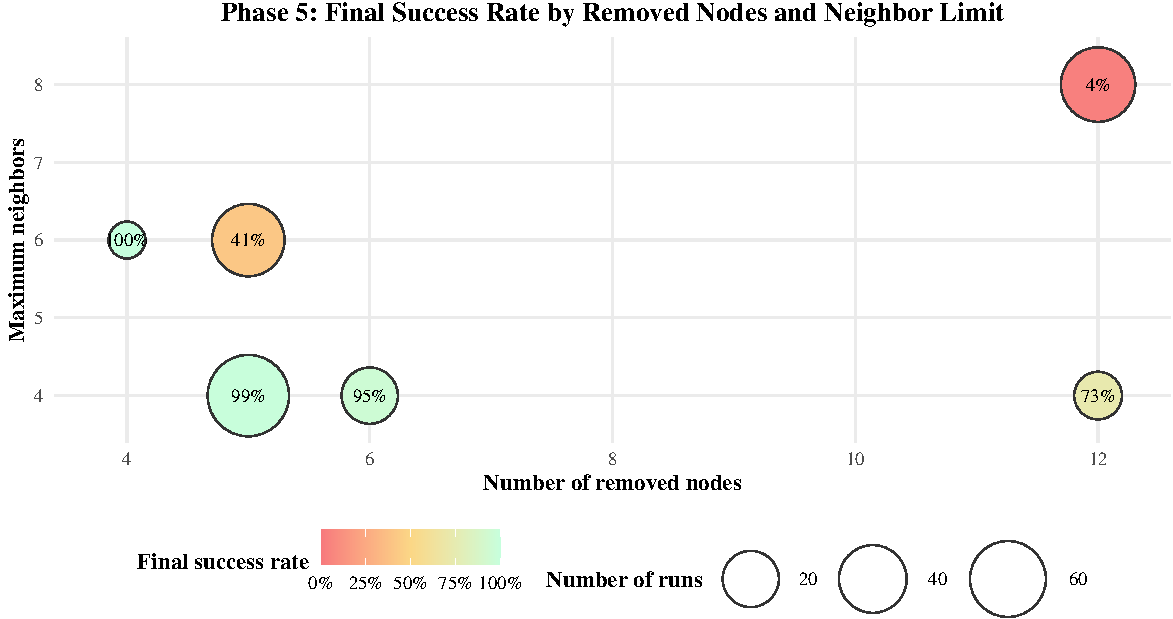
\includegraphics{figures/phase5-input-chart-1} \end{center}

\pandocbounded{\includegraphics[keepaspectratio]{http://127.0.0.1:39058/chunk_output/F9C83C15a463b8af/641E88A1/cgoaeoc4gw66d/000010.png}}

\subsection{Combined Input-Variable
Comparison}\label{combined-input-variable-comparison}

\begin{center}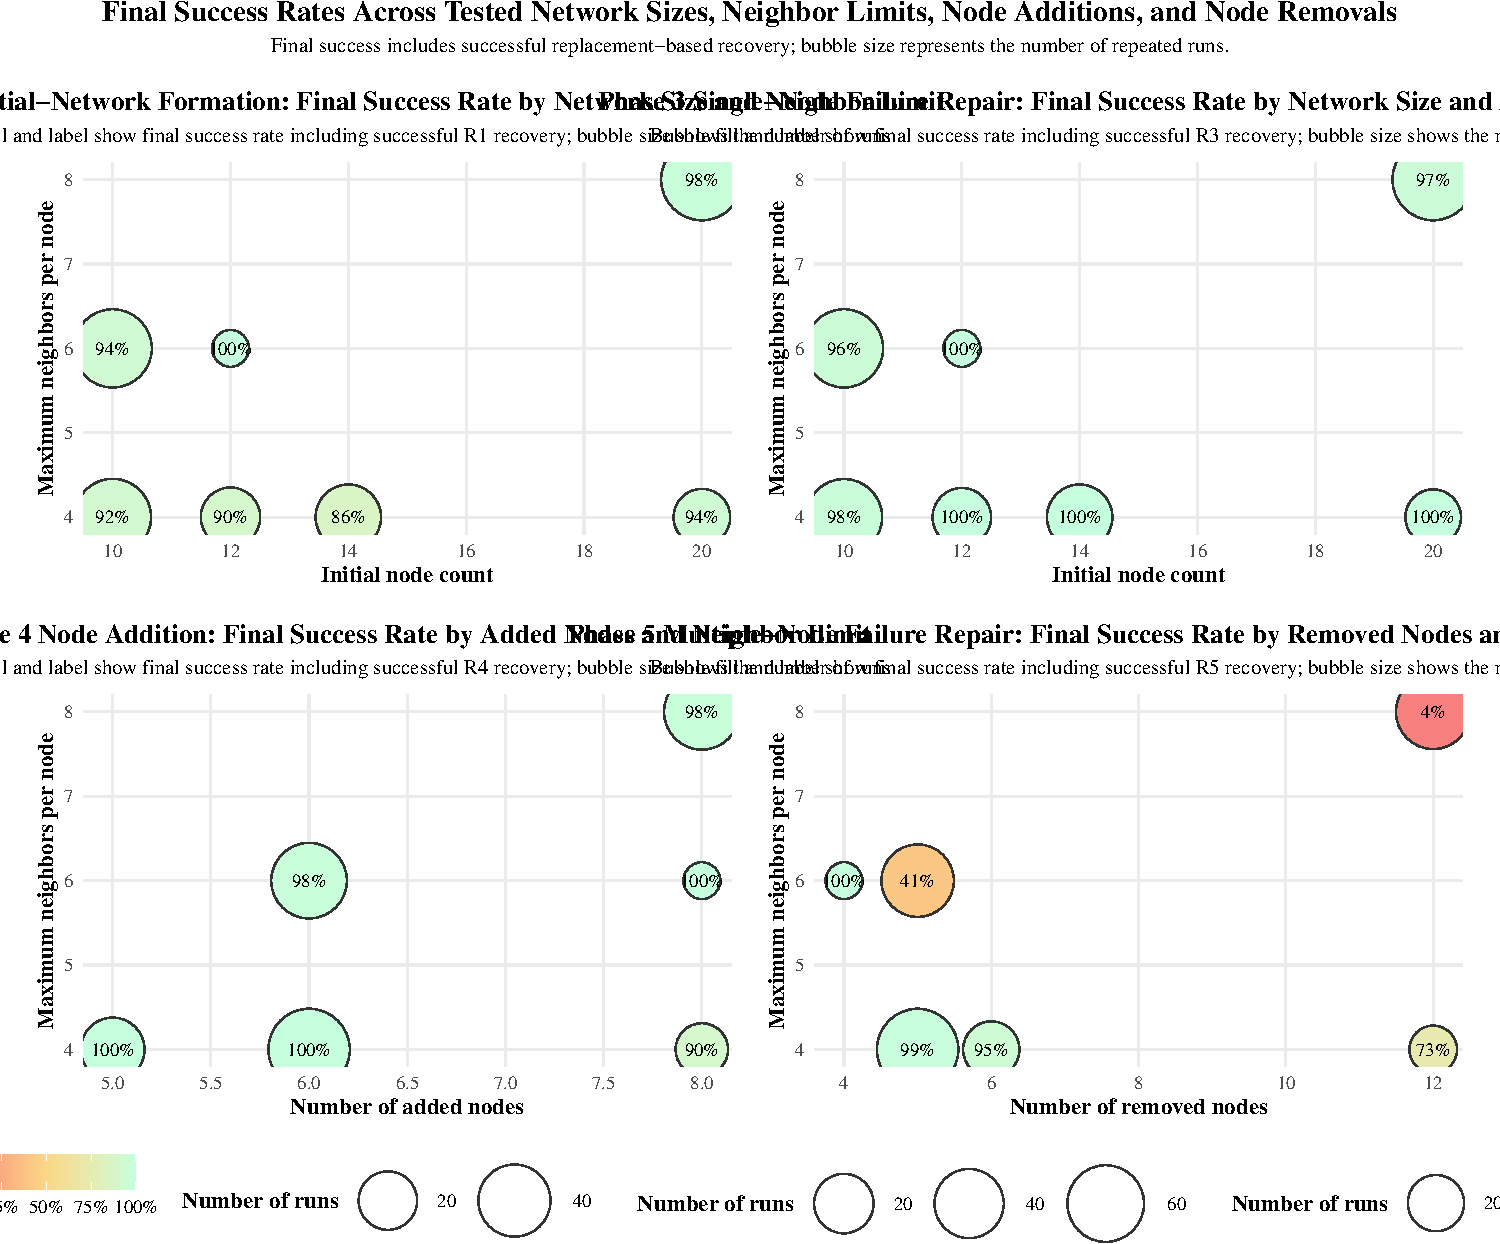
\includegraphics{figures/combined-input-chart-1} \end{center}

\section{Stability Checks}\label{stability-checks}

\begin{center}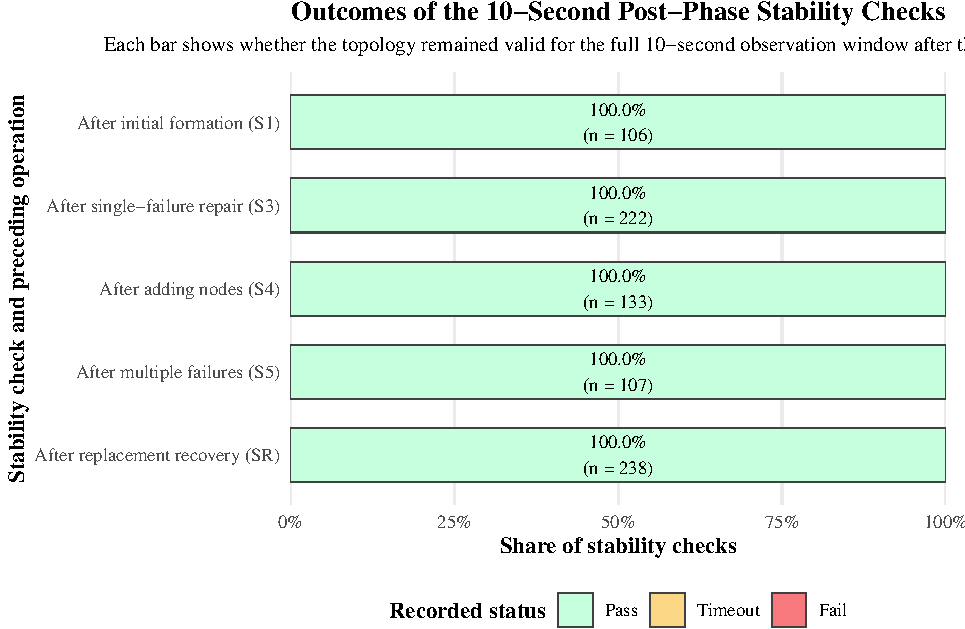
\includegraphics{figures/stability-success-chart-1} \end{center}

\section{Failure Detection Time}\label{failure-detection-time}

\begin{center}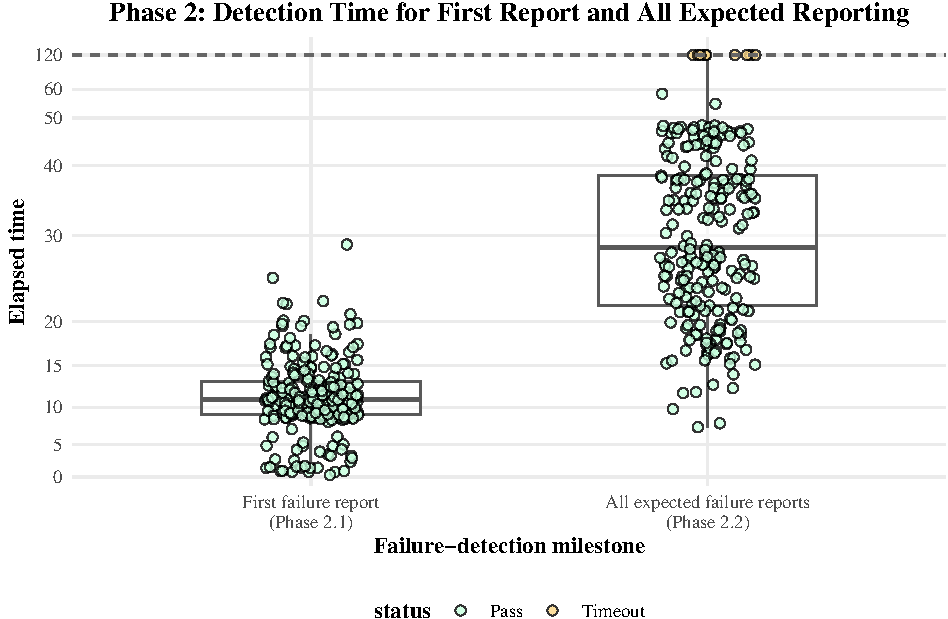
\includegraphics{figures/phase2-time-chart-1} \end{center}

\section{Main-Phase Completion Time and Input
Effects}\label{main-phase-completion-time-and-input-effects}

\subsection{Phase 1: Initial Network
Formation}\label{phase-1-initial-network-formation-1}

\begin{center}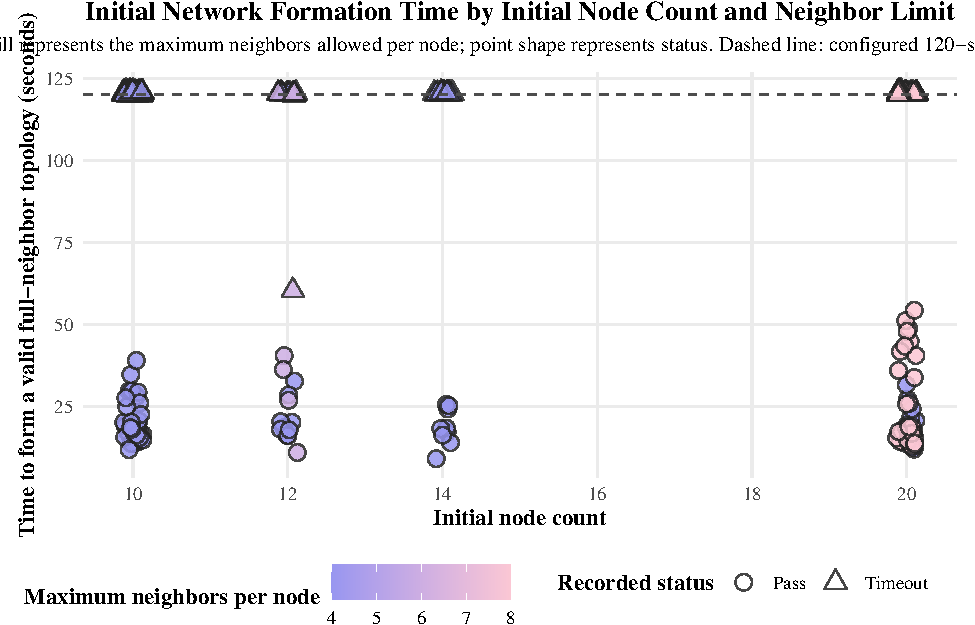
\includegraphics{figures/phase1-time-impact-chart-1} \end{center}

\subsection{Phase 3: Repair After One Node
Failure}\label{phase-3-repair-after-one-node-failure}

\begin{center}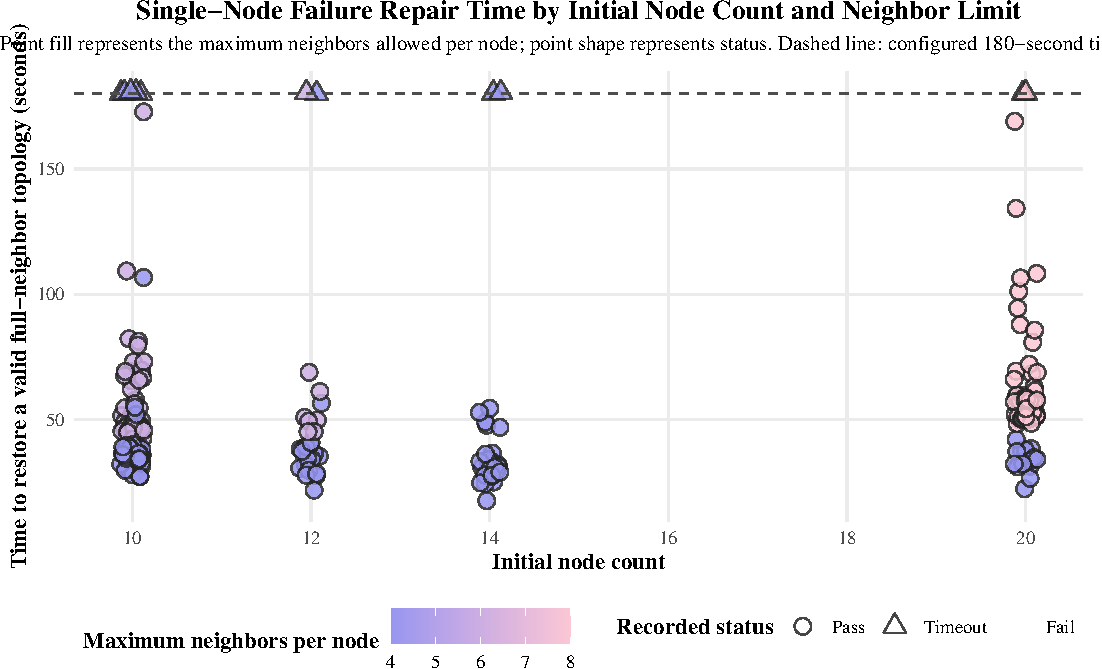
\includegraphics{figures/phase3-time-impact-chart-1} \end{center}

\subsection{Phase 4: Adding Nodes}\label{phase-4-adding-nodes-1}

\begin{center}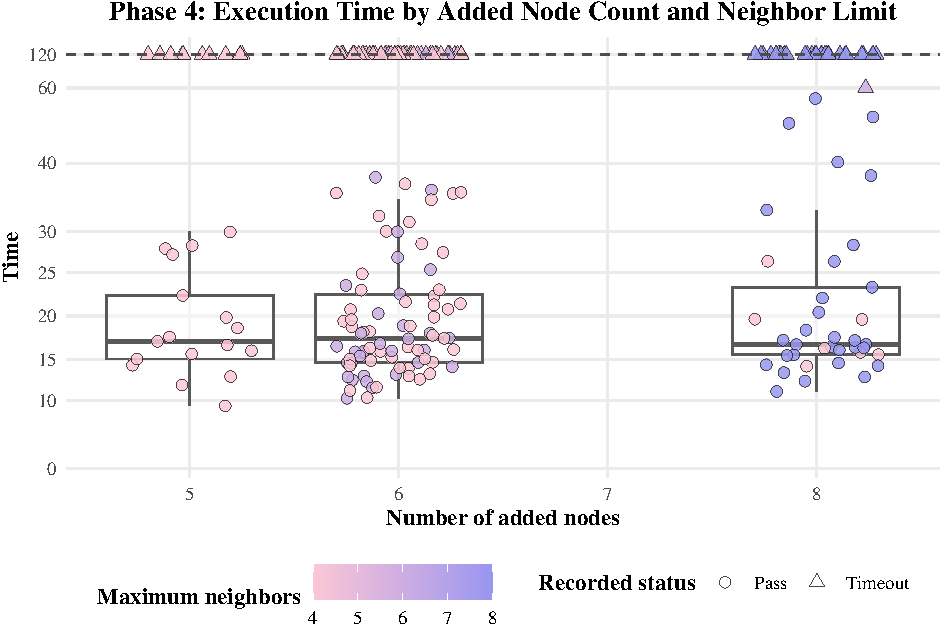
\includegraphics{figures/phase4-time-impact-chart-1} \end{center}

\subsection{Phase 5: Repair After Multiple Node
Failures}\label{phase-5-repair-after-multiple-node-failures}

\begin{center}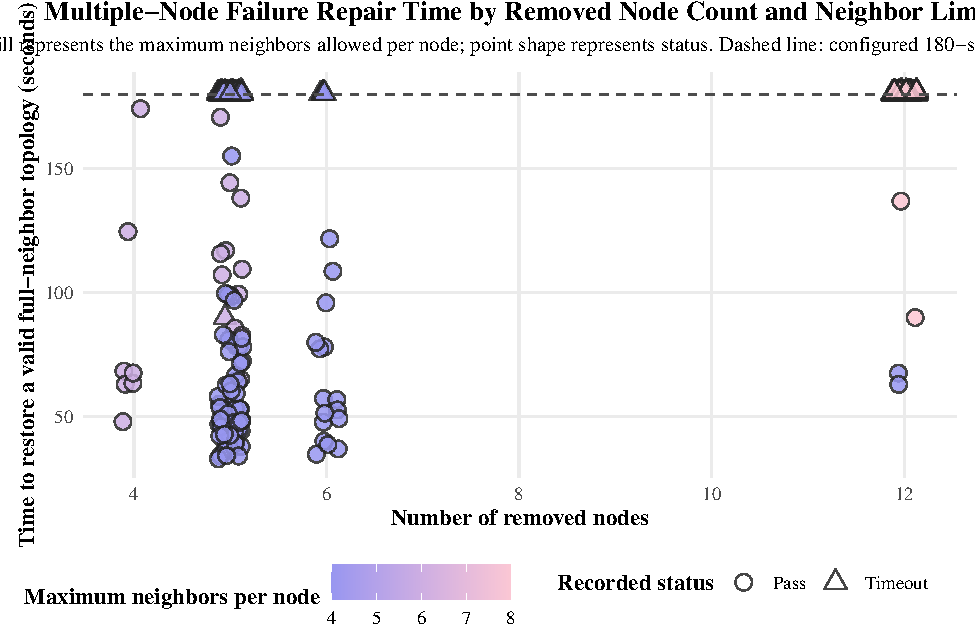
\includegraphics{figures/phase5-time-impact-chart-1} \end{center}

\section{Replacement-Based Recovery Completion
Time}\label{replacement-based-recovery-completion-time}

\begin{center}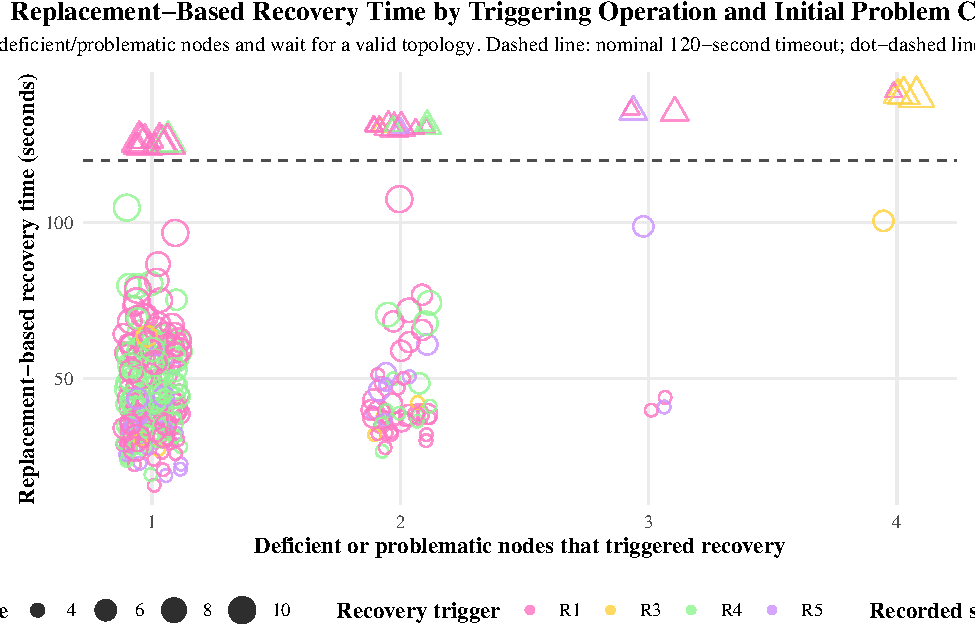
\includegraphics{figures/recovery-time-impact-chart-1} \end{center}

\section{Problematic Nodes in Failed Main
Phases}\label{problematic-nodes-in-failed-main-phases}

\subsection{Phase 1: Initial Network
Formation}\label{phase-1-initial-network-formation-2}

\begin{center}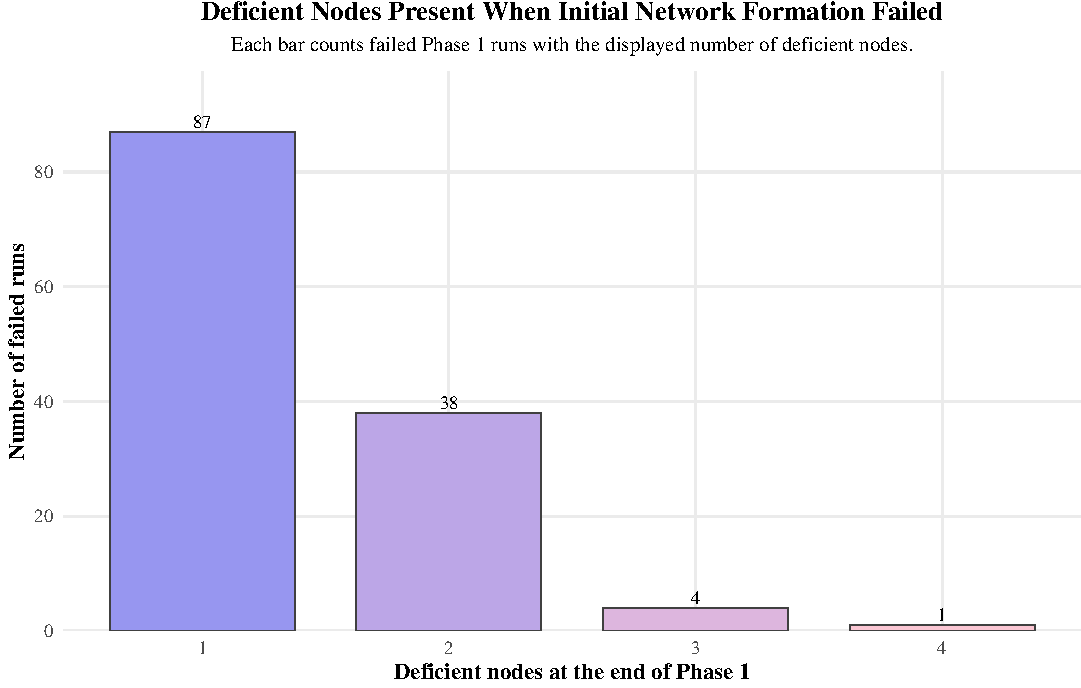
\includegraphics{figures/phase1-problem-count-chart-1} \end{center}

\subsection{Phase 3: Repair After One Node
Failure}\label{phase-3-repair-after-one-node-failure-1}

\begin{center}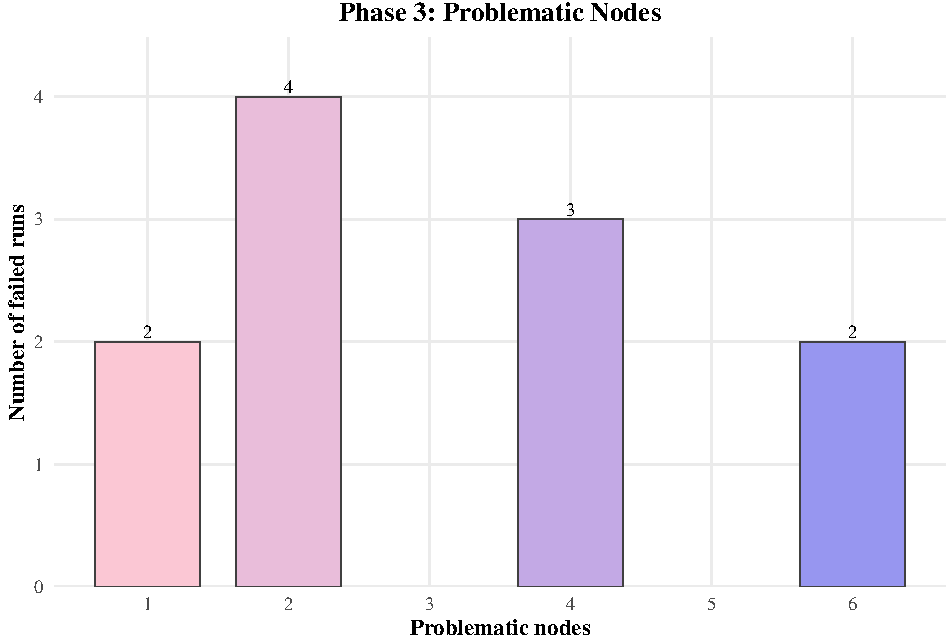
\includegraphics{figures/phase3-problem-count-chart-1} \end{center}

\subsection{Phase 4: Adding Nodes}\label{phase-4-adding-nodes-2}

\begin{center}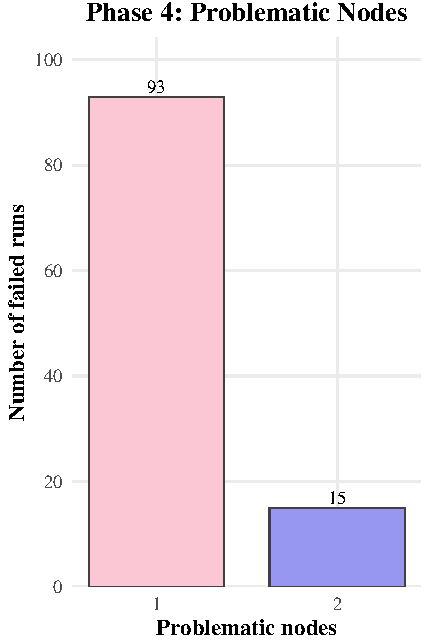
\includegraphics{figures/phase4-problem-count-chart-1} \end{center}

\subsection{Phase 5: Repair After Multiple Node
Failures}\label{phase-5-repair-after-multiple-node-failures-1}

\begin{center}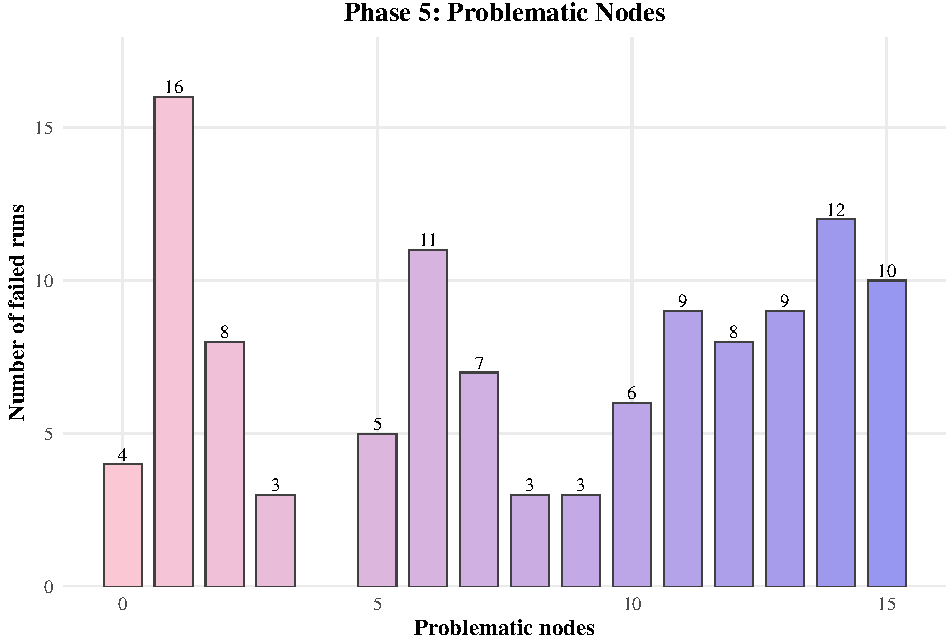
\includegraphics{figures/phase5-problem-count-chart-1} \end{center}

\section{Replacement-Based Recovery Success
Rates}\label{replacement-based-recovery-success-rates}

\begin{center}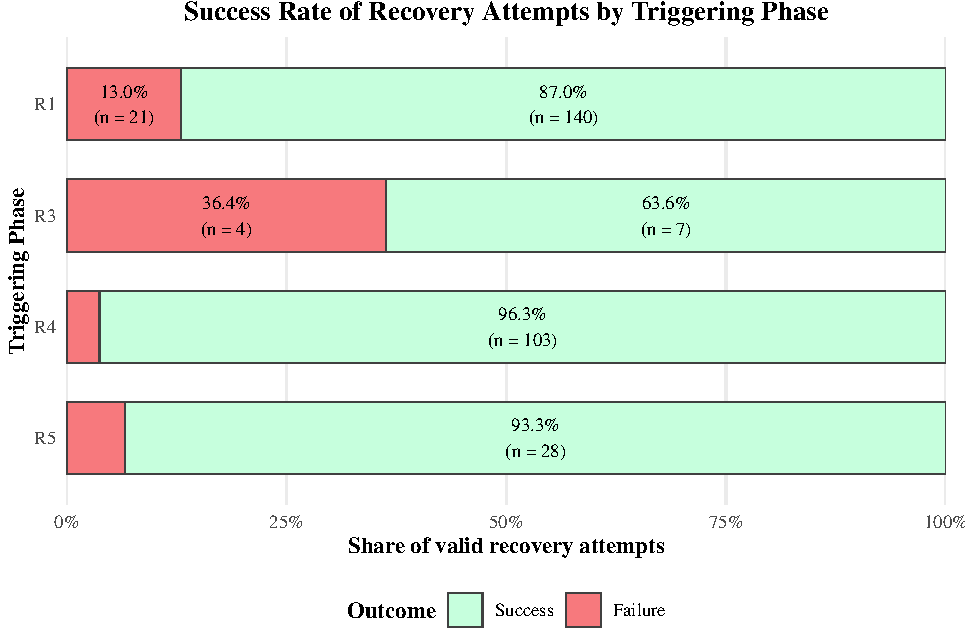
\includegraphics{figures/recovery-success-chart-1} \end{center}

\begin{longtable}[]{@{}lrrrrr@{}}
\caption{Valid replacement-based recovery attempts after timeout
filtering.}\tabularnewline
\toprule\noalign{}
phase & attempts & passes & timeouts & failures & success\_rate \\
\midrule\noalign{}
\endfirsthead
\toprule\noalign{}
phase & attempts & passes & timeouts & failures & success\_rate \\
\midrule\noalign{}
\endhead
\bottomrule\noalign{}
\endlastfoot
R1 & 130 & 115 & 15 & 0 & 0.885 \\
R3 & 9 & 6 & 3 & 0 & 0.667 \\
R4 & 94 & 92 & 2 & 0 & 0.979 \\
R5 & 27 & 25 & 2 & 0 & 0.926 \\
\end{longtable}

\end{document}
